\documentclass[a4,12pt]{book}
\usepackage[portuguese]{babel}
\usepackage[utf8]{inputenc}
\usepackage{graphicx}
\usepackage{amsmath,amssymb,amsthm}
\usepackage{tikz}

\newtheorem{example}{Exemplo}
\newtheorem{exercicio}{Exercício}
\newtheorem{definition}{Definição}
\newtheorem{theorem}{Teorema}

\newcommand{\xor}{\oplus}

%\newenvironment{proof}{{\em Demonstração:}}{\cqd\medskip}

\begin{document}

\bibliographystyle{alpha}

\author{Márcio Moretto Ribeiro}

\title{Segurança da Informação}

\maketitle

\chapter*{Apresentação}

Essas são notas de aula da disciplina Segurança da Informação ministrados no segundo semestre de 2017 para as turmas do período diurno e noturno do curso de Sistemas de Informação da Escola de Artes Ciências e Humanidades (EACH) da USP.
A primeira versão desta apostila foi escrita para o curso de verão ministrado entre os os dias 2 e 6 de fevereiro de 2015 também no campus leste da Universidade de São Paulo. 
O curso de verão foi oferecido como parte das atividades do projeto de Privacidade e Vigilância do Grupo de Políticas Públicas em Acesso à Informação (GPoPAI) e foi inspirado pelo curso online oferecido gratuitamente pela plataforma Coursera e ministrado pelo professor D. Boneh.

Aos alunos que pretendem se aprofundar no tema sugerimos as seguintes referências bibliográficas:

\begin{itemize}
\item J. Katz e Y. Lindell - {\em Introduction to Modern Cryptography}
\item W. Stallings - {\em Criptografia e Segurança da Informação}
\item C. Paar e J. Pelzl - {\em Understanding Cryptography}
\end{itemize}

Agradecemos aos alunos que participaram do curso de verão em 2015 e dos cursos de gradução em 2016 e 2017, suas contribuião serviram de importante feedback para escrita dessas notas.

Alguns direitos sobre o conteúdo desta apostila são protegidos pelo autor sob licença Creative Commons
Attribution-NonCommercial-ShareAlike 4.0 International (CC BY-NC-SA 4.0). Ou seja, você  é livre para distribuir cópias e adaptar este trabalho desde que mantenha a mesma licença, dê o devido crédito ao autor e não faça uso comercial.

\begin{center}
  
\includegraphics[width=.3\textwidth]{imagens/cc.png}
\end{center}
\chapter{Introdução}

\section{Privacidade}
\label{sec:privacidade}

As primeiras tentativas de conceitualizar a privacidade datam do final do século XIX.
Em um famoso artigo de 1890, os colegas da faculdade de direito de Bosto, Louis Brandeis e Samuel Warren denunciam que o advento da fotografia instantânea e o jornalismo haviam ``invadido o recinto sagrado da vida privada'' ferindo o que eles apontam como o direito individual de ``ser deixado em paz''.
Assim, eles argumentam que o escopo do direito comun ({\em Common Law}), que originalmente se concentrava apenas na proteção contra agreções e já havia sido ampliado para incluir a proteção à propriedade deveria ser novamente alargado para finalmente reconhecer a ``natureza espiritual do homem'' \cite{Warren1890}.

Essa visão da privacidade como proteção à intimidade ou, nas palavras dos autores, como o ``direito de ser deixado em paz'' é a chave de interpretação que prevalece no debate público.
Duas contribuições que não fogem a esse espírito, porém, merecem destaque nessas notas introdutórias.
Em um influente artigo de 1977, Richard Posner propõe que as disputas sobre direito à privacidade sejam interpretadas em sua dimensão econômica.
Para Posner, as informações privadas possuem valor. 
De um lado há o interesse de quem busca construir uma imagem pública sobre si, uma reputação e, de outro, há o interesse de se conhecer o outro para melhor saber como se relacionar com ele ou aprender sobre sua trajetória.
Caso fosse permitido qualquer tipo de intrusão à privacidade, o efeito seria um esforço maior em não revelar, ou inclusive não produzir, dados potencialmente valiosos.
Assim, a questão da privacidade, se resumiria a uma questão de eficiência econômica.
Caberia ao legislador regular o direito ao controle da reputação procurando um equilíbrio que maximizasse os fluxos de informação \cite{Posner77}. 

O risco tanto para o indivíduo cuja paz é  perturbada pelas fotos não autorizadas, quanto para aquele que perde o controle sobre sua reputação é de que algo que pertencia a sua esfera privada se tornasse pública.
Para Nissenbaum, essa dicotomização entre público e privado não dá conta dos problemas associados a quebra de privacidade.
Por exemplo, um paciente espera que as informações sobre sua condição de saúde sejam eventualmente compartilhadas com outros médicos ou médicas com o intuito de melhor diagnosticá-lo, assim como um cliente espera que seu gerente de banco use suas informações bancárias para sugerir-lhe melhores investimentos.
Porém, há uma flagrante quebra de privacidade se as informações médicas forem compartilhadas com o banco, com quem eventualmente o paciente negociará um plano de saúde.
Esse cenário exemplifica o que a autora chama de rompimento da ``integridade contextual do fluxo de informações'' \cite{Nissenbaum09}.

\section{Vigilância}
\label{sec:vigilancia}
% Foucalt e Deleuze

Associado ao tema da privacidade, mas ligado a outra matriz teórica, estão os debates sobre vigilância.
Diferente dos estudos sobre privacidade cujos principais autores são juristas preocupados com o direito individual, os esttudos sobre vigilância focam em relações de poder.
Foucault descreve a vigilância como uma técnica que teria alterado profundamente as formas de exercer o poder durante os séculos XVII e XIX.
O poder do senhor feudal durante a idade média era exercído por meio do suplício, a pena corporal em que o açoitado pedia misericórdia eventualmente concedida.
Após a revolução francesa o suplício foi sendo substituido pela prisão e aos poucos seria desenvolvida a técnica da disciplina e da vigilância.
Para o autor, a imagem que melhor descreve a técnica é uma estrutura arquitetônica proposta por Jeremy Bentham no final do século XVII.
Bentham arquitetou um modelo de prisão em que os vigias ficariam no centro aonde poderiam observar todas as celas, porém, aqueles que ocupam as celas não poderiam observar o vigia.
A sensação constante de estar sendo vigiado introgetaria a disciplina, outra técnica deste período, nos condenados.
O propósito da vigilância e da disciplina é o de produzir corpos dóceis e obedientes \cite{Foucault96}.

Em 1992, em um curto texto, Giles Deleuze propos uma atualização dos conceitos de Foucault que antecipariam o que hoje compreendemos como vigilância.
Na sociedade disciplinar, descrita por Foucault, durante a vida o indivíduos passa de uma instituição disciplinar a outra: da escola, ao exército, do exército à fábrica e da fábrica ao hospital.
Cada instituição disciplina o indivíduo e o modela da maneira mais eficiente à instituição.
Na sociedade do controle, conforme descrita por Deleuze, o poder é exercido de maneira mais intermitente e mais sutil.
O indivíduo prototípico da sociedade do controle seria o endividado cujo controle atravessa as instituições \cite{Deleuze92}.

\section{Marco Regulatório}
\label{sec:marco-regulatorio}
% Mayer-Schonberger

Antes ainda dos primeiros computadores, as chamadas máquinas Hollerith revolucioram a capacidade de processamento de dados.
Durante a década de trinta elas dinamizaram o processamento dos dados do censo nos EUA e na década de 40 foram usadas pelos nazistas para classificar aqueles, principalmente judeus, mas também comunistas e homossexuais, que deveriam ser transportados para os guetos, dos guetos para os campos de concentração e finalmente para as câmaras de gás \cite{Black01}.
Finda a guerra, a evolução dos modernos Estados de bem estar social Europeu e seu necessário processamento massivo de dados casou muito bem com o desenvolvimento computacional e assustou os cidadãos com sua centralidade de processamento.
Assim, começaram a surgir as primeiras leis de proteção de dados pessoais.

Mayer-Schonberger argumenta que, uma vez que as leis de proteção de dados pessoais na Europa partem todas das mesmas bases e diferem apenas em detalhes, é mais frutífero estudá-las em conjunto do que seguindo uma análise comparativa.
Ele propõe uma abordagem geracional como se existisse uma tendência evolutiva das normas.
A primeira geração, no começo dos anos 70, focou na regulamentação técnica dessas bases centralizadas de dados.
O surgimento de mini-computadores, que favorecia o processamento descentralizado, levou a uma adaptação na legislação.
A segunda geração, no final dos anos 70, focou na liberdade negativa, o direito civíl de "ser deixado em paz" nas palavras de Brandeis e Warren.
A autonomia do indivíduo é, porém, contraposta a sua inclusão nos programas sociais do Estado.
Então, a terceira geração legislativa, em meados dos anos 80, foge um pouco das liberdades negativas e foca em uma abordagem participativa de autodeterminação informacional.
A pergunta deixa de ser se alguém quer participar ou não de processos sociais, mas como.
Ainda assim, porém, os indivíduos estavam em uma posição frágil nas relações de negociação o que os levava, via de regra, a abdicar dos seus direitos.
A quarta geração, de meados dos ano 90, procurou de um lado equalizar as posições de negociação ainda apostando na autonomia do indivíduo, mas também incluiu diversos mecanismos mais paternalistas excluindo certas liberdades participativas e as sujeitando à proteção juridica obrigatória.
Nessa fase surgem órgãos de defesa, não apenas de auxílio aos cidadãos, mas com papel decisório para delibera contra violações \cite{Mayer-Schonberger97}.

No Brasil, o Marco Civil da Internet aprovado em 2013 não aborda diretamente as questões de proteção de dados pessoais.
Carecemos de um marco legal que imponha, pelo menos, que o uso de dados pessoas dependa necessariamente do consentimento explicito e informado e cuja autorização seja dada para um fim específico.

\section{Vigilância Digital em Massa}
\label{sec:vigil-digital}

Em 2013 Edward Snowden revelou ao mundo o alacance dos programas de vigilância em massas das agências de espionagem dos EUA.
O jornalista Glen Greenwald e a cineasta Laura Poitras divulgaram o caso em uma serie de matérias e um documentário \cite{Greenwald14, Poitras14}.
O vazamento demonstra que a agência de segurança nacional dos EUA (NSA) tem acesso a toda a comunicação por telefone e pelos principais meios de comunicação online do mundo.
O moderno modelo de negócios das empresas de internet baseado na propaganda direcionada depende da construção de perfis digitais que por sua vez dependem da produção e aquisição de uma grande escala dados pessoas.
Essa competição por dados pessoais cria o que chamamos de pontos únicos de falha.
A violação dessas bases permitiu à NSA produzir um banco de dados pesquisável da agência possui toda comunicação pública e privada que passa pelos servidores da Google, do Facebook, da Microsof e da Apple.

A vigilância digital em massa eleva o problema da privacidade para um outro patamar.
Não se trata apenas de proteger a intimidade, ou a inviolabilidade do lar, ou do controle na construção da reputação. 
Nesse contexto, o problema da privacidade é também coletivo.
A privacidade deve ser também enchergada como um direito civil, uma limitação ao poder do estado de antecipar as ações de grupos políticos. 
Para tanto, é preciso de ação politica de concientização, de regulamentação para restringir o poder das empresas que controlam o armazenamento dos dados pessoais e também desnvolvimento técnico. 

\section{Segurança da Informação}
\label{sec:seg-inf}

A internet é um meio intrinsecamente promíscuo \cite{}.
Por uma decisão de projeto, não temos controle por onde nossas informações passam quando nos comunicamos pela rede.
Conforme produzimos mais informações pessoais e permitimos que elas circulem, maior o risco de quebra da integridade dos fluxos contextuais.
Em particular há atores poderosos com capacidade conhecida de observar a comunicação em escala global o que traz um risco coletivo tanto à soberania nacional dos países perifércos, como o Brasil, quanto à democracia.
A regulamentação, absolutamente necessaria para controlar minimamente esses processos e garantir pelo menos o consentimento no uso de nossas informações pessoais, certamente não é suficiente.
A compreensão, o desenvolvimento e a difusão de ferramentas de segurança da informação podem colaborar nesse sentido.
Concluiremos o capítulo com uma história motivadora.

Após as denúncias de Snowden houve uma espécie de consenso nos meios ativistas sobre a importância de focar forças em desenvolver ferramentas que garantissem a criptografia ponta a ponta.
O paradigma mais comum de comunicação na rede é criptografar a comunicação entre cada cliente e o servidor.
Como já dissemos, conforme poucos servidores consentram a maior parte da comunicaçõ online, a informação armazenada nesses servidores passa a ser um bem muito requisitado.
A ideia para superar isso seria criptografar a comunicação entre clientes.
Assim, a informação armazenada nos servidores não seria compreensível seja pelos engenheiros das empresa que controla a comunicação, seja para um ator externo como um hacker ou a NSA.
O principal protocolo de criptografia ponta a ponta na época era o PGP, que havia sido criado no começo da década de 90, antes do advento da web.
As tentativas mal sucedidas de ressucitar o protocolo logo foram substituídas por um esforço em atualizá-lo.
Duas aplicações que garantiam criptografia ponta a ponta em celulares se popularizaram nesse período: Telegram e o Textsecure.
A primeira foi desenvolvida por uma compania russa e oferece serviço de criptografia ponta a ponta em comunicação síncrona usando um protocolo desenvolvido por seus engenheiros.
A segunda foi desenvolvida por uma pequena empresa no Vale do Silício e se inspirou no protocolo OTR, que por sua vez se inspirou no PGP, adaptando-o para o contexto assíncrono mais adequado para a comunicação móvel.
Os esforços de ativistas em promover esse tipo de ferramenta culminou com a adoção do protocolo do Textsecure, rebatizado como Signal, no Whatsapp, a ferramenta de comunicação móvel mais usada no mundo todo.
A popularização da criptografia ponta a ponta em grande parte da comunicação interpessoal muda muito o cenário de proteção de direitos civis e de liberdade de organização.
É certo que os metadados das comunicações - quem fala com quem, quando e de onde - não estão protegidos, é certo que a maior parte da comunicação interpessoal não está livre de intrusão seja de hackers, seja de agências governamentais, é certo que há serviços - como agenda online - em que simplesmente não há alternativa segura e, portanto, é necessaria muita ação política e desenvolvimento técnico nessa área.
\chapter{Cifras Clássicas}
\label{cha:cifras-classicas}

Como argumntamos no primeiro capítulo, a internet é um meio de comunicação promíscuo.
As partes que se comunicam pela rede não tem controle sobre por quais caminhos sua comunicação irá trafegar.
Essa característica, porém, não se restringe a esse meio.
Durante o século XVIII, por exemplo, toda correspondência que passava pelo serviço de correios de Viena na Austria era encaminhada para um escritório -- {\em black chamber} -- que derretia o selo, copiava seu conteúdo, recolocava o selo e reincaminhava para o destinatário.
Todo esse processo durava cerca de três horas para não atrasar a entrega.
Como a Áustria, todas as potências européias desse período operavam suas {\em back-chambers}.
As invenções do telegrafo e do rádio só facilitaram a capacidade de criar grampos, no primeiro caso, ou simplesmente captar a comunicação no segundo \cite{Kahn96}.

Partiremos, portanto, do seguinte modelo de comunicação.
Duas partes, o remetente e o destinatário, buscam se comunicar.
Tradicionalmente denominaremos o remetente de Alice e o destinatário de Bob.
Nossa suposição principal é que o canal de comunicação entre as partes é inseguro.
Ou seja, assumiremos que terceiros, que denominaremos de Eva, são capazes de observar as mensagens que trafegam pelo canal de comunicação.
Essa suposição é conhecida em alguns meios como ``hipótese da comunicação hacker''.
Para efeitos deste curso, sempre assumiremos essa hipótese.

A {\em criptografia} (do grego ``escrita secreta'') é a pratica e o estudo de técnicas de comunicação segura na presença de terceiros chamados de {\em adversários}.
A {\em criptoanálise}, por sua vez, é o estudo e a análise dos sistemas de informação com a intenção de desvelar seus segredos.
Nosso primeiro desafio no curso é apresentar sistemas de comunicação que garantam a {\em confidencialidade}.
Ou seja, toda mensagem enviada de Alice para Bob deve ser compreensível apenas para Alice e Bob e deve ser incompreensível para Eva:
\begin{center}
\begin{tikzpicture}[node distance=2cm,auto,>=latex]
\node (alice) {Alice};
\node (bob) at (10,0) {Bob};
\node (eva) at (5,2) {Eva};
\draw[->] (alice) -> node[above]{mensagem} (bob);
\path[->] (eva) edge (5,.5);
\end{tikzpicture}
\end{center}

Se a importância da comunicação confidencial entre civis tem se tornado cada vez mais urgente, no meio militar é difícil remontar suas origens. 
Suetônio (69 - 141) por volta de dois mil anos atrás descreveu como o imperador Júlio César (100 a.c. - 44 a.c.) escrevia mensagens confidenciais:


\begin{quote}
  ``Se ele tinha qualquer coisa confidencial a dizer, ele escrevia cifrado, isto é, mudando a ordem das letras do alfabeto, para que nenhuma palavra pudesse ser compreendida. 
  Se alguém deseja decifrar a mensagem e entender seu significado, deve substituir a quarta letra do alfabeto, a saber 'D', por 'A', e assim por diante com as outras.''
\end{quote}

O esquema que chamaremos de cifra de César é ilustrado pelo seguinte exemplo:

\begin{verbatim}
Mensagem: transparenciapublicaopacidadeprivada
Cifra:    XUDQVSDUHQFLDSXEOLFDRSDFLGDGHSULYDGD
\end{verbatim}

Como descrito Suetônio, a regra para encriptar uma mensagem consiste em substituir cada letra da mensagem por aquela que está três posições a sua frente na ordem alfabética.
Para descriptografar a cifra, substituir cada letra por aquela que está três posições atrás.
O problema com este tipo de sistema é que basta conhecer a regra de criptografia para decifrá-lo.
Em outras palavras, o segredo da cifra é sua própria regra.
 
Embora técnicas de criptografia e criptoanálise existam desde o império romano, foi com o advento do teléfgrafo e sua capacidade de comunicação eficiente, que o campo se estruturou.
No fim do século XIX Auguste Kerckhoff estabeleceu seis princípios que as cifras militares deveriam satisfazer:
\begin{enumerate}
\item O sistema deve ser indecifrável, se não matematicamente, pelo menos na prática.
\item O aparato não deve requerer sigilo e não deve ser um problema se ele cair nas mãos dos inimigos.
\item Deve ser possível memorizar uma chave sem ter que anotá-la e deve ser possível modificá-la se necessário.
\item Deve ser possível aplicar a sistemas telegráficos.
\item O aparato deve ser portátil e não deve necessitar de muitas pessoas para manipulá-lo e operá-lo.
\item Por fim, dadas ascircunstâcias em que ele será usado, o sistema deve ser fácil de usar e não deve ser estressante usá-lo e não deve exigir que o usuário conheça e siga uma longa lista de regras.
\end{enumerate}

O segundo princípio ficou conhecido como {\em princípio de Kerckhoff}.
Ele estabelece que a regra usada para criptografar uma mensagem, mesmo que essa regra esteja codificada em um mecanismo, não deve ser um segredo e não deve ser um problema caso ela caia nas mãos do adversário.
Nas palavras de Claude Shannon: ``o inimigo conhece o sistema''.
Whitfield Diffie coloca o debate nos seguintes termos:

\begin{quote}
``Um segredo que não pode ser rapidamente modificado deve ser interpretado como uma vulnerabilidade''
\end{quote}

Ou seja, em uma comunicação confidencial as partes devem compartilhar algo que deve ser ``possível de modificar caso necessário''.
Esse segredo compartilhado é o que chamaremos de {\em chave} da comunicação e assumiremos que ela é a única parte sigilosa do sistema.
Trazendo o debate para uma discução mais moderna, o sigilo do código-fonte de um sistema não deve em hipótese alguma ser aquilo que garanta sua segurança.

O modelo de {\em criptografia simétrica}, portanto, pode ser descrito da seguite maneira:
o remetente usa um algoritmo público ($E$) que, dada uma chave ($k$), transforma uma mensagem ($m$) em um texto incompreensível chamado de {\em cifra} ($c$), a cifra é enviada para o destinatário por um meio assumidamente inseguro (hipótese da comunicação hacker) e o destinatário utiliza a mesma chave em um algoritmo ($D$) que recupera a mensagem a partir da cifra.

\begin{center}
\begin{tikzpicture}[node distance=2cm,auto,>=latex]
\node (alice) at (0, 2){Alice};
\node (bob) at (10, 2) {Bob};
\node (eva) at (5, 2) {Eva};

\node (m1) at (0,1) {$m$};
\node (k1) at (0,-1) {$k$};
\node (E)  at (2,0) {$E(k,m) = c$};
\node (D)  at (8,0) {$D(k,c) = m$};
\node (k2) at (10,-1) {$k$};
\node (m2) at (10,1) {$m$};

\path[->] (eva) edge (5,1);
\draw[->] (m1) -> (E);
\draw[->] (k1) -> (E);
\draw[->] (D) -> (m2);
\draw[->] (k2) -> (D);
\draw[->] (E) -> node[above]{$c$} (D);
\end{tikzpicture}
\end{center}

\section{Cifra de Deslocamento}
\label{sec:cifra-deslocamento}

O que chamamos na seção anterior como ``cifra de César'' não deve ser propriamente considerado uma cifra, pois não possui uma chave.
Porém, é possível e simples adaptar esse esquema para incorporar uma chave.
Para tanto faremos a seguinte alteração no esquema.
Ao invés de deslocar as letras sempre três casas para frente vamos assumir que foi sorteado previamente um número $k$ entre $0$ e $23$.
Esse número será a chave da comunicação e, portanto, assumiremos que as partes a compartilham.
O mecanismo para criptografar uma mensagem será o de deslocar cada letra $k$ posições para a direita e para descriptografá-la basta deslocar cada letra as mesmas $k$ posições para a esquerda.

Para formalizar este mecanismo vamos assumir que cada letra do alfabeto seja representada por um número: a letra {\tt a} será representada pelo $0$, a letra {\tt b} pelo $1$ e assim por diante.
O universo de todas as chaves possíveis é o conjunto $K = \{0 ... 23\}$ (chamaremos este conjunto de $\mathbb{Z}_{26}$ ou de maneira mais genérica $\mathbb{Z}_n = \{0, 1, \dots, n - 1\}$) e o universo de todas as mensagens possíveis é representado pelo conjunto $M = {\mathbb{Z}_{26}}^\star$, ou seja, todas as sequências de números entre $0$ e $23$.
Além disso, o conjunto das possíveis cifras é $C = M$.
Precisamos descrever três algorítmos:
\begin{itemize}
\item $Gen$ que gera a chave $k \in K$,
\item $E$ que recebe uma chave $k \in K$ e uma mensagem $m \in M$ e produz uma cifra $c \in C$ (i.e.: $E: K \times M \to C$) e
\item $D$ que recebe uma chave $k \in K$ e uma cifra $c \in C$ e produz uma mensagem $m \in M$ (i.e.; $D: K \times C \to M$).
\end{itemize}

Um sistema de criptografia simétrica $\Pi$ é formado por essa tripla de algoritmos $\Pi = \langle Gen, E, D \rangle$.
Além disso, precisamos garantir que quem possui a chave seja capaz de descriptografar a cifra.
Ou seja, precisamos garantir que:
\begin{displaymath}
  D(k, E(k, m)) = m
\end{displaymath}

O mecanismo que gera uma chave na cifra de substituição é bastante simples, ele simplesmente sorteia com uma distribuição de probabilidade uniforme um número entre $0$ e $23$.
Escreveremos da seguinte forma:
\begin{displaymath}
Gen := k \leftarrow \mathbb{Z}_{26}  
\end{displaymath}

Utilizaremos a partir daqui a convenção de usar uma seta da direita para esquerda indicando que será escolhido um elemento do conjunto com probabilidade uniforme.

O algoritmo para criptografar uma mensagem traz um pequeno problema.
Escreveremos $m = m_0 m_1 m_2 \dots m_n$ uma mensagem $m$ com $n + 1$ letras cuja primeira letra é $m_0$, a segunda é $m_1$ e assim por diante.
Nossa primeira tentativa de formalizar $E$ seria somar $k$ a cada uma das letras $m_i$.
O problema é que esta soma pode resultar em um valor que não corresponde a nenhuma letra i.e. $m_i + k > 23$.
Para evitar este problema utilizaremos não a aritmética convencional, mas a {\em aritmética modular}.

Dizemos que um número $a$ divide $b$ (escrevemos $a|b$) se existe um número inteiro $n$ tal que $a.n = b$.
Dois números são equivalentes módulo $n$ (escrevemos $a \equiv b\ (mod\ n)$) se $n|(b-a)$.
Em outras palavras, dois números são equivalentes módulo $n$ se o resto da divisão de cada um por $n$ for o mesmo reultado.
O conjunto de todos os números equivalentes módulo $n$ forma uma classe de equivalência que representaremos como $[a\ mod\ n] = \{b \in \mathbb{Z} : a \equiv (b\ mod\ n)\}$.
Por exemplo $[5 + 7\ mod\ 10] = [2\ mod\ 10]$ pois $5 + 7 = 12$ e o resto de $12$ por $10$ é $2$.

Estamos finalmente em condições de formalizar o sistema da cifra de deslocamento $\Pi = \langle Gen, E, D\rangle$:
\begin{itemize}
\item $Gen := k \leftarrow \mathbb{Z}_{26}$
\item $E(k, m) = [m_0 + k\ mod\ 26] \dots [m_n + k\ mod\ 26]$
\item $D(k, c) = [c_0 - k\ mod\ 26] \dots [c_n - k\ mod\ 26]$ 
\end{itemize}


\begin{example}
  Considere a palavra {\tt XUXA}.
  Usando a cifra de César com chave $k = 3$ obtemos a cifra {\tt BZBD}.

  \begin{itemize}
  \item $E(3, \textrm{\tt 24 21 24 0}) = [1\ mod\ 26] [21\ mod\ 26] [1\ mod\ 26] [3\ mod\ 26]$  
  \item $D(3, \textrm{\tt 1 21 1 3}) = [24\ mod\ 26] [21\ mod\ 26] [24\ mod\ 26] [0\ mod\ 26]$
  \end{itemize}

  Note que $[27\ mod\ 26] = [1\ mod\ 26]$ e que $[-2\ mod\ 26] = [24\ mod\ 26]$.
\end{example}



\section{Cifra de Substituição}
\label{sec:cifra-monoalfabetica}

Em 1567 a residência da rainha da Mary da Escócia foi destruída por uma explosão que levou a morte do então rei, primo de Mary.
O principal suspeito do assinato foi dispensado da pena e se casou com Mary no mês seguinte.
O episódio levou-a a prisão na Inglaterra.
Neste tempo, para a maioria dos católicos, Mary era a legítima herdeira do trono inglês - ocupado pela protestante Elizabeth I.
Durante o tempo na prisão Mary consiporou com aliados pela morte de Elizabeth.
Em 1587 Mary foi executada pelo que ficou conhecido como a conspiração de Babington.
A principal prova utilizada para a condenação foi uma troca de cartas cifradas interceptadas e decifradas \cite{Singh04}.

A cifra usada pelos conspiradores é conhecida hoje como {\em cifra de substituição} ou {\em cifra monoalfabética}.
Neste tipo de criptografia, cada letra ou par de letras é substituída por um símbolo, que pode ser inclusive uma outra letra.
Assim, a chave desse tipo de cifra é um alfabeto.


\begin{example}
  Considere a seguinte chave de uma cifra monoalfabética.
  Neste caso os símbolos utilizados letras do mesmo alfabeto em ordem embaralhada:
  \begin{verbatim}
    Alfabeto:   abcdefghijklmnopqrstuvwxyz
    Permutação: ZEBRASCDFGHIJKLMNOPQTUVWXY
  \end{verbatim}

  A partir desta chave podemos produzir textos substituindo cada letra pela letra correspondente na chave.
  Para descriptografar, basta fazer o processo inverso, a saber, substituir a letra da cifra pela do alfabeto.
  
  \begin{verbatim}
    Mensagem: transparenciapublicaopacidadeprivada
    Cifra:    QOZKPMZOAKBFZMTEIFBZLMZBFRZRAMOFUZRZ
  \end{verbatim}
\end{example}

O desfecho da história da conspiração de Babington sugere que a cifra monoalfabética não é muito segura.
De fato, no próximo capítulo discutiremos melhor as técnicas de criptonálise para este tipo de cifra.
Não obstante, até o desenvolvimento das primeiras máquinas de criptografar, versões das cifras monoalfabéticas foram eram as cifras mais populares no mundo todo.
Nos anos 70 a editora abril publicou no Brasil o famoso Manual do Escoteiro Mirim da Disney que apresentava uma cifra monoalfabética.
Mais recentemente, o curioso caso do desaparecimento de um rapaz no Acre viralizou quando seus familiares revelaram que no seu quarto havia uma coleção de livros que ele havia escrito de maneira criptografada.
Mais tarde foi descoberto que o rapaz usara uma cifra de substituição cuja chave foi eventualmente encontrada.

Para fechar esta seção buscaremos formalizar o sistema de cifra de substituição simples.
Uma {\em permutação} sobre um conjunto $\Sigma$ qualquer é uma {\em função bijetora} $p: \Sigma \to \Sigma$.
Funções bijetoras possuem a característica de serem inversíveis, ou seja, existe $q: \Sigma \to \Sigma$ tal que $p(q(x)) = q(p(x)) = x$.
A função $q$ é chamada de {\em inversa} de $p$, é única e será representada como $p^{-1}$.
O conjunto de todas as permutações, todas as funções bijetoras, de $\Sigma$ será representado como $Perm(\Sigma)$.
A chave de uma cifra de substituição é uma permutação do alfabeto $\mathbb{Z}_{26}$ escolhida aleatoriamente.
Para encriptar uma mensagem basta aplicar essa permutação a cada uma das mensagens e para descriptografá-la basta aplicar a função inversa.

Formalmente temos que $\Pi = \langle Gen, E, D \rangle$ em que:
\begin{itemize}
\item $Gen := k \leftarrow Perm(\mathbb{Z}_{26})$
\item $E(k, m) = k(m_0) \dots k(m_n)$
\item $D(k, c) = k^{-1}(c_0) \dots k^{-1}(c_n)$
\end{itemize}

\section{Cifra de Vigenère}
\label{sec:cifra-de-vigenere}

A cifra de Vigènere foi criada no século XV e ainda no começo do século XX era considerada inquebrável -- em 1868 o matemático e autor de Alice no País das Maravilhas, descreveu a cifra como ``inquebrável'' e um artigo da Scientific American de 1917 a descrevia como ``impossível de traduzir''.
Veremos no próximo capítulo que há um exagero nessas descrições, porém, a sofisticação desse tipo de cifra chamado de {\em polialfabética} tornava sua criptoanálise muito mais sofisticado.

Em poucas palavras, a cifra de Vigenère consiste em deslocar as letras do texto original em distâncias diferentes.
Em sua versão mais simples, sua chave consiste de uma palavra cuja primeira letra indica quantas casas devemos deslocar a primeira letra da mensagem, a segunda letra da chave indica quantas casa devemos deslocar a segunda letra e assim por diante.
Quando a mensagem ultrapassa o tamanho da chave, repetimos a chave e continuamos o processo.

Para facilitar a conta na hora de criptografar e descriptografar, podemos usar uma tabela que indica para cada letra da mensagem e cada letra da chave qual é a letra correspondente na cifra.
Essa tabela é chamada de {\em tabula recta} e está representada na Figura \ref{fig:tabula-recta}.

\begin{figure}[htbp]
  \centering
  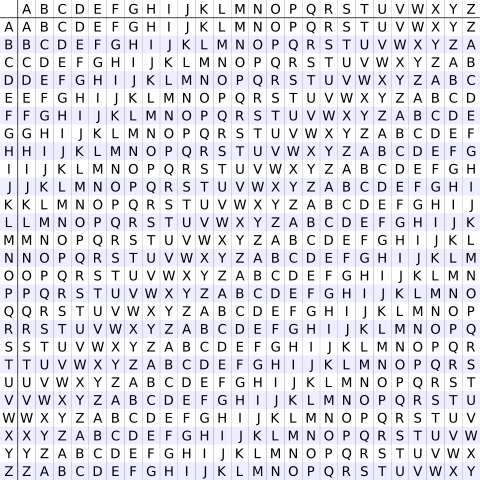
\includegraphics[width=.8\textwidth]{imagens/tabula-recta.png}
  \caption{Tabula Recta}
  \label{fig:tabula-recta}
\end{figure}


\begin{example}
  Considere a seguinte mensagem criptografada com a chave {\tt senha} usando a cifra de Vigenère:

\begin{verbatim}
Mensagem: transparenciapublicaopacidadeprivada
Chave:    senhasenhasenhasenhasenhasenhasenhas
Cifra:    LVNUSHEELNUMNWUTHVJAGTNJIVEQKPJMIHDS
\end{verbatim}  
\end{example}

Para fechar o capítulo vamos fazer o exercício de formalizar a cifra de Vigenère.
A chave consiste em uma sequência de letras, tipicamente escolhidas em um dicionário, mas vamos aqui supor que a escolha seja aleatória e com um tamanho fixado $l$.
A partir dessa semente, podemos gerar uma chave auxiliar $k'$ obtida repetindo $k$ quantas vezes forem necessárias até que $|k'| = |m| = n$.
Para criptografar basta desolcar $m_i$ por $k_i'$ posições.
Formalmente temos que $\Pi = \langle Gen, E, D \rangle$

\begin{itemize}
\item $Gen := k \leftarrow \mathbb{Z}_{26}^l$
\item $E(k, m) = [m_0 + {k_0}'\ mod\ 26] \dots [m_n + {k_n}'\ mod\ 26]$
\item $D(k, c) = [c_0 - {k_0}'\ mod\ 26] \dots [c_n - {k_n}'\ mod\ 26]$
\end{itemize}

\section{Maquinas de Criptografar}
\label{sec:maquinas}

No final da primeira década do século XX foram inventadas as primeiras máquinas de criptografar.
A componente principal dessas {\em maquinas eletromecânicas} é um conjunto de {\em rotores}.
A configuração inicial dos rotores contém a chave da criptografia.
Cada vez que o operador pressiona uma tecla o rotor embaralha as letras.
Dessa forma, essas {\em máquinas rotoras} se comportam como uma sofisticada cifra polialfabética.
Para descriptografar a mensagem, o operador precisa ajustar a máquina em modo de descriptografia, ajustar a configuração inicial com a chave secreta e digitar o texto cifrado.
A máquina então irá se rearrajar para produzir o texto original quando digitado.

As máquinas rotora mais conhecida são da série {\em Enigma}.
Elas foram criadas por um inventor alemão no final da primeira guerra mundial e versões mais modernas foram extensamente usadas durante a segunda guerra pelo exército nazista.
As versões mais simples da máquina possuiam três rotores capazes de gerar $26^3$, ou cerca de $175$ mil possíveis configurações iniciais.
Além disso, era possível trocar a ordem dos rotores multiplicando por $6$ o número de combinações possíveis e chegando a um total de cerca de $105$ mil possibilidades.
A versão utilizada pelo exercito nazista, porém, permitia cerca de $150$ trilhões de possibilidades.
Em 1939 Alan Turing desenvolveu uma máquina eletromecânica chamada {\em Bombe} capaz de decifrar algumas cifras de máquinas Enigma com 3 rotores e, posterioirmente foi melhorada para decifrar mensagens de máquinas Enigma mais sofisticadas.

A história da computação esbarra na história da criptografia neste ponto.
Poucos anos antes da guerra, Alan Turing demonstrara que a satisfatibilidade da lógica de primeira ordem é um {\em problema indecidível}.
Para tanto ele propôs um {\em modelo computacional} que hoje chamamos de {\em Máquinas de Turing}.
Diferente dos modelos computacionais anteriores como o {\em cálculo lambda} de Church ou as {\em funções recursivas} de Gödel, o modelo de Turing era intuitivo.
Além disso, Turing mostrou que era possível construir com seu modelo uma {\em Máquina Universal} capaz de simular qualquer outra Máquina de Turing.
Esse resultado magnífico é o que dá origem a computação.
O primeiro modelo de computador desenvolvido por Turing e sua equipe em Bechley Park foi batizado de {\em Colossus} e tinha como principal propósito quebrar outra cifra usada pelos nazistas durante a guerra, a {\em cifra de Lorenz}.
A cifra de Lorenz é uma versão do que estudaremos com o nome de {\em cifra de fluxo}.
Para decifrar os códigos das máquinas Enigma e da cifra de Lorenz os ingleses tiveram que contar, não apenas com o texto criptografado que interceptavam sem grandes dificuldades, mas também com uma série cifras cujas mensagens eles conheciam previamente.
Veremos mais pra frente a importância desta informação. 
A capacidade dos aliados de decifrar as mensagens de seus adversários foi central para sua vitória. 

O começo do século XX marcou o surgimento das primeiras máquinas de criptografar, as primeiras máquinas de criptoanálise. 
Na metade do século começaram a surgir os primeiros computadores.
Nos anos 70 a comunicação seria revolucionada pelo advento da internet, mas antes disso já ficara claro que era necessário compreender melhor o que faz uma cifra ser segura. 
\chapter{Criptoanálise}
\label{cha:criptoanalise}

Nos capítulos anteriores vimos uma série de cifras que a história deu conta de mostrar que não são seguras.
Neste capítulo focaremos nas técnicas para quebrar essas cifras.
O estudo e a análise dos sistemas de informação com a intenção de desvelar seus segredos é o que chamamos de {\em criptoanálise}.

\section{Ataques Força Bruta}
\label{sec:forca-bruta}

Uma forma universal de quebrar uma cifra é conhecido como {\em ataque força bruta}.
Ele consiste no seguinte procedimento.
O adversário utiliza o esquema $D$, que sempre assumimos ser de conhecimento público, numa cifra $c$ com uma primeira tentativa de chave $k_0$ para produzir $D(k_0, c) = m_0$.
A mensagem $m_0$ provavelmente não fará nenhum sentido, então o adversário repete o processo com uma outra chave $k_1$ e em seguida com $k_2$ e assim por diante até que mensagem produzida seja coerente.

Consideremos a cifra de deslocamento.
Estabelecemos que uma chave nesse tipo de sistema é escolhida aleatoriamente no conjunto $\mathbb{Z}_{26}$.
Assim existem exatamente 26 possibilidades de chave, porque $|\mathbb{Z}_{26}| = 26$.
O número esperado de tentativas até se encontrar a chave procurada é $\frac{|K|}{2}$, neste caso 13.
Ou seja, a cifra de deslocamento é muito vulnerável a ataques de força bruta porque seu universo de chaves é extremamente pequeno.

Em contraste vamos calcular o universo de chaves da cifra de substituição.
Vimos que o universo das chaves de uma cifra de susbstituição é $Perm(\mathbb{Z}_{26})$.
Calcular $|Perm(\mathbb{Z}_{26})|$ é um exercício simples de {\em análise combinatória}.

\begin{eqnarray*}
  |Perm(\mathbb{Z}_{26}|) & = & 26!\\
                         & = & 26.25.24 \dots 1\\
                         & \approx & 4.10^{26}\\
                         & \approx & 2^{88}
\end{eqnarray*}

O universo de chaves na cifra de deslocamento é tão pequeno que é possível testar na mão todas as possibilidades de chaves.
Certamente não é possível testar as possibilidades de chaves da cifra de substituição na mão.
Ataques força bruta, porém, são facilmente automatizáveis.
Voltaremos a pergunta sobre o tamanho do universo de chaves para uma comunicação segura no capítulo \ref{chap:senhas}.


\begin{example}
Muitos dos roteadores modernos possuem um mecanismo chamado de WPS (Wi-Fi Protected Setup) que supostamente simplificaria o processo de conexão, especialmente na configuração do hardware.
O WPS permite que um usuário se conecte remotamente e sem fio no roteador desde que possua um PIN (Personal Identification Number).
Esse PIN é uma sequência de oito digitos de 0 a 9.
Ou seja, o universo das chaves é $10^8 \approx 2^{27}$.
Neste contexto, um ataque força-bruta é possível e toma entre 4 e 8 horas.  
\end{example}


\section{Ataques de Frequência}
\label{sec:frequencia}

A cifra de substituição é suficientemente segura contra ataques de força-bruta.
Como vimos, porém, ela não é tão segura quanto a rainha Mary da Escócia gostaria.
A forma como os funcionários da rainha Elizabeth quebraram a cifra de substituição é o que chamamos de {\em ataque de frequência}.
A ideia por trás desse tipo de ataque é bastante simples.
Na cifra de substituição, cada letra é substituída por um símbolo.
Portanto, a frequência de cada símbolo em um texto suficientemente longo deve ser parecida com a frequência média de cada letra naquela língua.
Por exemplo, no português, esperamos que os símbolos mais comuns sejam o {\tt a}, o {\tt e} e o {\tt o}.
Para piorar -- ou melhorar dependendo da perspectiva -- na maioria das línguas há digrafos particulares, por exemplo, no português dois símbolos repetídos provavelmente representam o {\tt r} ou o {\tt s} e o {\tt h} quase sempre vem depois do {\tt l} ou do {\tt n}.
Se o texto a ser decifrado for suficientemente longo, essas pistas podem ser suficientes para quebrar a cifra.

No seguinte trecho de ``O escaravelho de ouro'' de Edgar Allan Poe a personagem descreve essa técnica que ela utilizou para decifrar um texto em inglês \cite{}:

\begin{quote}
``Ora, no inglês, a letra que ocorre com mais frequência é a letra {\tt e}. 
Depois dela, a sucessão é: {\tt a o i d h n r s t u y c f g l m w b k p q x z}. 
O e prevalece de tal maneira que quase nunca se vê uma frase isolada em que ele não seja predominante. 
Aqui nós temos, portanto, bem no início, uma base que permite mais do que um mero palpite. 
O uso que se pode fazer da tabela é óbvio, mas, neste criptograma em particular, não precisamos nos valer dela por inteiro. 
Como nosso caractere dominante é o {\tt 8}, começaremos assumindo que este é o {\tt e} do alfabeto normal. (...)''
\end{quote}

Em português, faz sentido separar as letras em cinco blocos, com frequência de ocorrência decrescente:
\begin{enumerate}
\item {\tt a}, {\tt e} e {\tt o}
\item {\tt s}, {\tt r} e {\tt i}
\item {\tt n}, {\tt d}, {\tt m}, {\tt u}, {\tt t} e {\tt c}
\item {\tt l}, {\tt p}, {\tt v}, {\tt g}, {\tt h}, {\tt q}, {\tt b} e {\tt f}
\item {\tt z}, {\tt j}, {\tt x}, {\tt k}, {\tt w} e {\tt y}
\end{enumerate}

\section{Ataques à ``Cifra Invencível''}
\label{sec:criptoanalise-vegenere}

Apesar da fama de ``inquebrável'' que a cifra de Vigenère oustentou até o começo do século XX, desde a metade do século anterior já eram conhecidos métodos de criptoanálise capazes de detorratar esse tipo de cifra.
Em 1854 John Hall Brock Thwaites submeteu um texto cifrado utilizando uma cifra supostamente por ele inventada.
Charles Babbage, o inventor das máquinas que precederam o computador moderno, mostrou que no fundo a cifra de Thwaites era equivalente a cifra de Vigenère.
Após ser desafiado, Babbage, decifrou uma mensagem criptografada por Thwaites duas vezes com chaves diferentes.

Em 1863 Friedrich Kasiski formalizou um ataque contra a cifra de Vigenère que ficou conhecido como {\em teste de Kasiski}.
O ataque considera o fato de que a chave se repete com uma frequência fixa e, portanto, há uma probabilidade de produzir padrões reconhecíveis.
Considere o exemplo extraído da Wikipédia:

\begin{example}
\begin{verbatim}
Mensagem: cryptoisshortforcryptography
Chave:    abcdabcdabcdabcdabcdabcdabcd
Cifra:    CSASTPKVSIQUTGQUCSASTPIUAQJB
\end{verbatim}  
\end{example}

Note que o padrão CSASTP se repete na cifra.
Isso ocorre porque o prefixo {\tt crypto} foi criptografado com a mesma chave.
Uma vez encontrado um padrão como este, é calculada a distância entre as repetições.
Neste caso a distância é 16, o que significa que o tamanho da chave deve ser um divisor de 16 (2, 4, 8 ou 16).
Com esta informação, podemos aplicar um ataque de frequência nos caracteres de 2 a 2, de 4 a 4, de 8 a 8 e de 16 a 16.

\section{Exercícios}
\label{sec:exercicios}


\begin{exercicio}
Calculo o tamanho do universo das chaves em uma cifra de Vigenère da forma como usada normalmente (escolhendo um palavra) e na forma como apresentamos formalmente (sequência aleatória com tamanho fixo $l$)?  
\end{exercicio}


\begin{exercicio}
Construa um script que extraia um corpus do português moderno (por exemplo, textos da wikipedia) e calucule a frequência de ocorrência das letras do alfabeto. 
\end{exercicio}

\begin{exercicio}
Em 2017 um rapaz que ficou conhecido como menino do Acre ficou dias desaparecido e deixou uma serie de livros criptografados com cifra de substituição em seu quarto.
A Figura \ref{fig:menino-do-acre} está reproduzida uma página de um desses livros. 
Utilize a análise de frequência para decifrar o texto.
\end{exercicio}

\begin{figure}[htbp]
  \centering
  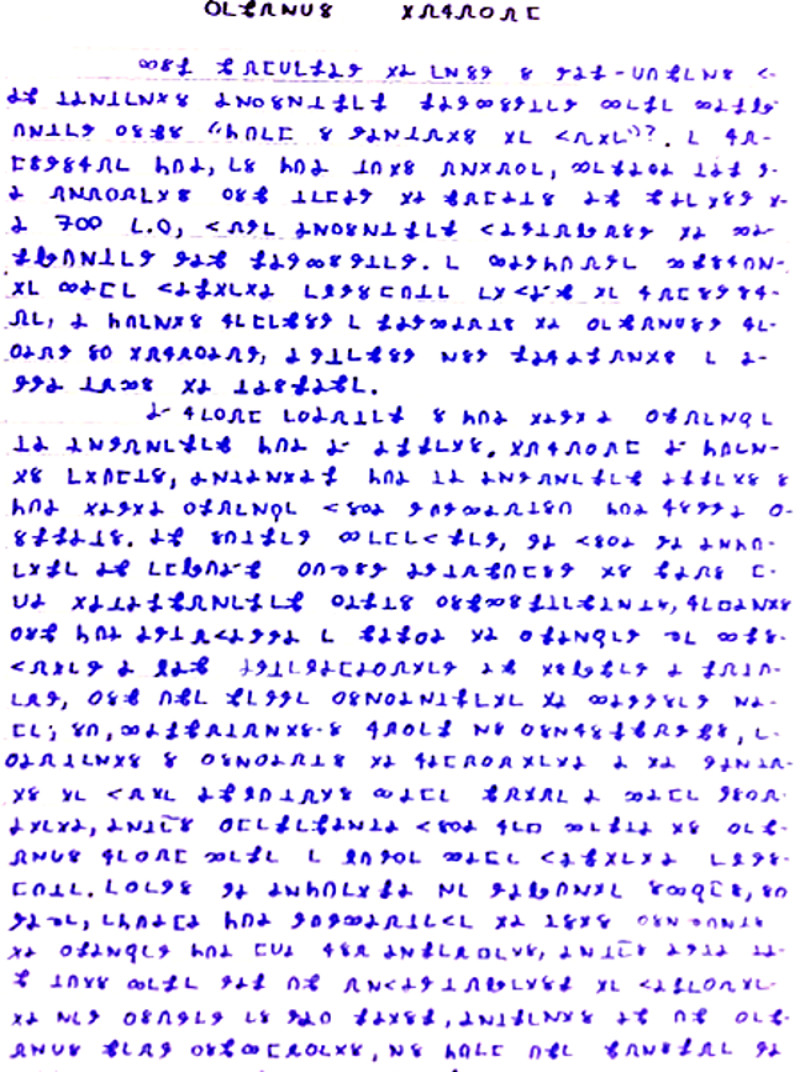
\includegraphics[width=.8\textwidth]{imagens/bruno.jpg}
  \caption{Texto criptografado pelo Menino do Acre}
  \label{fig:menino-do-acre}
\end{figure}

% Colocar aqui a frequência das letras em portugês, de preferência com um gráfico
% Inserir o exemplo do menino do Acre a partir do trabalho que eles enviarem
% Técnica para quebrar a cifra de Vigenère


\chapter{Sigilo Perfeito}
\label{cha:sigilo-perfeito}

No final dos anos 40, com o desenvolvimento dos primeiros computadores e a experiência da quebra das cifras mecanicamente produzidas por poderosas máquinas desenvolvidas pelo esforço de guerra do nazismo, alguns cientístas se voltaram para um problema central no campo da criptografia: o que torna um sistema de criptografia seguro?
As cifras que vimos até agora são conhecidas como ``cifras clássicas'' extamente porque elas precedem desse debate moderno, e não a toa foram todas derrotadas cedo ou tarde.
Informalmente, poderíamos dizer que o problema dos esquemas clássicos de criptografia é que eles guardam muita informação sobre a mensagem (frequência das letras, dos dígrafos, letras duplas etc.). 
Não é uma coincidência, portanto, que a primeira tentativa de formalizar o conceito de segurança tenha sido proposto por Claude Shannon, o fundador da teoria da informação.
Shannon definiu o que hoje chamamos de {\em sigilo perfeito}.
Um esquema de criptografia garante o sigilo perfeito se a cifra não guarda nenhuma informação sobre a mensagem que a gerou.
Ou, de maneira um pouco mais descritiva, se a probabilidades da cifra ocorrer é independente da probabilidade da mensagem:

\begin{definition}
  Um esquema de criptografia simétrica $\Pi = \langle Gen, E, D \rangle$ garante o {\em sigilo perfeito} se, supondo que $Pr[C=c] > 0$, para toda distribuição de probabilidade sobre $M$ temos que:
\begin{displaymath}
  Pr[M = m | C = c] = Pr[M = m]
\end{displaymath}

Ou de maneira equivalente se para todo $m_0, m_1 \in M$ e todo $c \in C$ temos que:
\begin{displaymath}
  Pr[C = c | M = m_0] = Pr[C = c | M = m_1]
\end{displaymath}
\end{definition}

Essa segunda formulação é mais intuitiva, ela estabelece que um sistema garante o sigilo perfeito se a probabilidade de $m_0$ produzir a cifra $c$ é idêntica a probabilidade de qualquer outra mensagem $m_1$ produzir a mesma cifra $c$.
O exemplo a seguir mostra que a cifra de substituição não garante o sigilo perfeito:

\begin{example}
  Seja $\Pi = \langle Gen, E, D \rangle$ o sistema de criptografia de substituição e sejam $c = \textrm{\tt ANA}$, $m_0 = \textrm{\tt OVO}$ e $m_1 = \textrm{\tt EVA}$.
Como o sistema $\Pi$ substitui cada letra da mensagem por uma letra na cifra, existem chaves $k$ tal que $E(k, m_0) = c$ -- basta que $k(\textrm{\tt O}) = \textrm{\tt A}$ e $k(\textrm{\tt V}) = \textrm{\tt N}$, de fato a chance de escolher uma chave assim é $\frac{1}{26^2} = \frac{1}{676}$ --, mas não existe nenhuma chave $k'$ tal que $E(k', m_1) = c$.
Portanto temos que:
\begin{displaymath}
Pr[C = c | M = m_0] =  \frac{1}{676} \neq Pr[C = c | M = m_1] = 0  
\end{displaymath}
\end{example}

Uma forma equivalente, e útil como veremos mais para frente, de definir sigilo perfeito é a partir de um jogo.
Imaginamos que há um adversário $\mathcal{A}$ cujo objetivo é quebrar a cifra produzida pelo sistema $\Pi$.
O jogo funciona da seguinte maneira: $\mathcal{A}$ escolhe duas mensagens $m_0$ e $m_1$ com o mesmo tamanho ($|m_0| = |m_1|$) e envia para o sistema $\Pi$.
O sistema gera uma chave $k$ usando o algoritmo $Gen$ e sorteia aleatoriamente uma das mensagens para criptografar ($\Pi$ sorteia $b \leftarrow \{0, 1\}$ e criptografa $m_b$).
A cifra produzida $E(k, m_b) = c$ e enviada de volta para o adversário, cujo desafia é acertar qual das duas mensagens foi cifrada.
O diagrama abaixo ilustra o processo:

\begin{center}
\begin{tikzpicture}[node distance=2cm,auto,>=latex]
\tikzset{
  player/.style={draw,shape=rectangle,rounded corners,minimum width=4em,minimum height=6em}
}
\node[player] (system) {$\Pi$};
\node[player] (adversary) at (10,0) {$\mathcal{A}$};
\draw[->] (9,.5) -> node[above]{$m_0, m_1 \in M : |m_0| = |m_1|$} (1,.5);
\draw[->] (1,-.5) -> node[above]{$E(k,m_b) = c$} (9,-.5);
\draw[->] (0,2) -> node{$b \leftarrow \{0,1\}$} (system);
\draw[->] (adversary) -> node{$b' \in \{0,1\}$} (10,-2);
\end{tikzpicture}
\end{center}

Chamamos o experimento ilustrado pelo diagrama de $PrivK^{eav}_{\Pi, \mathcal{A}}$.
Os subscritos indicam que o experimento depende do sistema $\Pi$ e do adversário $\mathcal{A}$.
O resultado do experimento deve ser $0$ se o adversário perdeu o desafio e $1$ caso contrário.
Formalmente temos que:
\begin{displaymath}
  PrivK^{eav}_{\Pi, \mathcal{A}} = \left\{
    \begin{array}{lcl}
      1 & \textrm{se} & b = b'\\
      0 & \textrm{c.c.} &\\
    \end{array}
    \right.
\end{displaymath}

É possível provar que um sistema $\Pi$ garante o {\em sigilo perfeito} se e somente se para qualquer adversário $\mathcal{A}$ temos que:
\begin{displaymath}
Pr[PrivK^{eav}_{\Pi, \mathcal{A}} = 1] = \frac{1}{2}
\end{displaymath}

Em palavras, o sistema possui sigilo perfeito se nenhum adversário é capaz de acertar qual ads mensagens produziu a cifra $c$ com probabilidade melhor do que um meio.

\section{One Time Pad}
\label{sec:otp}

Temos agora uma definição formal de segurança.
Vimos que a cifra de substituição não satisfaz essa definição, mas na verdade nenhuma das cifras clássica a satisfaz.
Não seria desejável que essas cifras satisfizessem a definição, pois vimos no capítulo anterior que nenhuma das cifras clássicas é segura e todas podem ser derrotadas se o adversário tiver acesso a uma cifra de tamanho suficientemente grande.
Ficamos então com o desafio de encontrar algum sistema que satisfaça essa definição, caso tal sistema exista.

No que segue apresentaremos um sistema chamado {\em One Time Pad} (OTP), também conhecida como {\em cifra de Vernan}, e mostraremos que ele garante o sigilo perfeito.
A partir deste ponto, conforme começaremos a investigar sistemas a serem implementados computacionalmente, consideraremos que o espaço $M$ das mensagens (assim como o espaço $C$ das cifras) será representado como sequências de bits.
No caso específico do OTP assumiremos que as mensagens e a cifras possuem um tamanho fixo $n$.
Mais importante é o fato de que o universo das chaves é também um conjunto de sequências de bits do mesmo tamanho.
Assim temos que $M = C = K = \{0,1\}^n$.
O sistema $\Pi = \langle Gen, E, D \rangle$ é definido pelos seguintes algoritmos:
\begin{itemize}
\item $Gen := k \leftarrow \{0,1\}^n$
\item $E(k,m) = [m_0 + k_0\ mod\ 2] \dots [m_n + k_n\ mod\ 2] = m \xor k$
\item $D(k,c) = [c_0 + k_0\ mod\ 2] \dots [c_n + k_n\ mod\ 2] = c \xor k$
\end{itemize}

Para verificar a corretude do sistema basta notar que:

\begin{eqnarray*}
  D(k, E(k, m)) & = & D(k, k \xor m)\\
                & = & k \xor (k \xor m)\\
                & = & (k \xor k) \xor m\\
                & = & m
\end{eqnarray*}

A derivação usa o fato de que a operação de {\em ou exclusivo} $\xor$ é associativa, que $x \xor x = 1$ e $1 \xor x = x$ para todo sequência de bits $x \in \{0,1\}^*$.
Deixamos como exercício mostrar essas três propriedades da operação.

\begin{example}
  Considere uma mensagem $m = 101010$ e uma chave $k = 010001$.
Usando o sistema One Time Pad a cifra produzida é a seguite:

\begin{displaymath}
  \begin{array}{ccccc}
    m & \xor & k & = & c \\
    101010 & \xor & 010001 & = & 111011
  \end{array}
\end{displaymath}
\end{example}

Como antecipado, é possível, e relativamente simples provar que o OTP possui sigilo perfeito.

\begin{theorem}
  O sistema de criptografia {\em One Time Pad} possui sigilo perfeito.
\end{theorem}

\begin{proof}
  Seja $K = M = C = \{0,1\}^n$.
  Dada uma cifra $c \in C$ e uma mensagem qualquer $m \in M$, existe uma única chave $k \in K$ tal que $E(k,m) = c$.
  A chave é exatamente $k = m \xor c$, pois:
  
  \begin{eqnarray*}
    E(k, m) & = & k \xor m \\
            & = & (m \xor c) \xor m\\
            & = & (m \xor m) \xor c\\
            & = & c
  \end{eqnarray*}

Como existe exatamente uma chave possível que faz com que $E(k,m) = c$, temos que a probabilidade se produzir $c$ dado uma mensagem qualquer $m$ é igual a probabilidade de sortear uma chave específica no universo $K = \{0,1\}^n$ que é $\frac{1}{2^n}$:
\begin{displaymath}
  Pr[C = c | M = c] = \frac{1}{2^n}
\end{displaymath}

Essa probabilidade é idêntica para qualquer $m \in M$.
Portanto, temos que $Pr[C = c| M = m_0] = Pr[C = c | M = m_1] = \frac{1}{2^n}$. 
\end{proof}

O {\em One Time Pad} possui duas severas limitações.
A primeira é indicada pelo próprio nome do sistema.
A sistema supõe que a chave de criptografia $k$ seja usada exatamente uma vez (``one time'').
Caso o mesmo $k$ seja usada para criptografar duas mensagens distintas $m_1$ e $m_2$, o sistema se torna completamente inseguro.

Para ilustrar essa limitação considere que duas cifras $c_0$ e $c_1$ foram produzidas usando a mesma chave $k$.
Assim temos que $c_0 = k \xor m_0$ e $c_1 = k \xor m_1$.
Note o que acontece quando aplicamos o ou exclusivo entre as duas cifras eliminamos a chave:


\begin{eqnarray*}
  c_0 \xor c_1 & = & (k \xor m_0) \xor (k \xor m_1)\\
              & = & (k \xor k) \xor (m_0 \xor m_1)\\
              & = & m_0 \xor m_1
\end{eqnarray*}

Uma vez eliminada a chave, é fácil separar as mensagens $m_0$ de $m_1$ utilizando um técnica similar ao ataque de frequência.

A segunda e mais crítica limitação do OTP é o tamanho de sua chave.
A suposição que fizemos é que o tamanho da chave deve ser tão grande quanto a mensagem a ser cifrada.
Há uma série de problemas práticos com isso.
Computacionalmente não é possível gerar chaves aleatórias muito grandes, o que limita o tamanho das mensagens que podemos cifrar.
Além disso, assumimos que as chaves são compartilhadas entre as partes.
Deixamos os detalhes sobre a distribuição de chaves para o capítulo \ref{}, mas por ora podemos adiantar que se nossa chave é tão grande quanto a mensagem, porque não enviamos a mensagem pelo mesmo canal que enviaríamos a mensagem?
Enfim, um sistema cuja a chave seja tão grande quanto a mensagem é de muito pouca utilidade prática.

Encerramos este capítulo mostrando que esta segunda limitação do OTP infelizmente não é uma peculiaridade do sistema.
Na verdade todo sistema que possua sigilo perfeito está fadado a ter chaves tão grandes o maiores do que a mensagem.
Esse resultado negativo foi proposto e demonstrado pelo próprio Shannon ainda nos anos 40.


\begin{theorem}[Teorema de Shannon]
Seja $\Pi = \langle Gen, E, D \rangle$ um sistema que garante o sigilo perfeito, então temos que $|K| \geq |M|$.  
\end{theorem}
\begin{proof}
  Consideraremos $M(c)$ como o conjuto de todas as mensagens que podem produzir $c$, ou seja, as mensagens $m \in M$ tal que $E(k, m) = c$ para algum $k \in K$.
  É claro que $|M(c)| \leq |K|$.
  Agora suponha por absurdo que $|K| < |M|$.
  Neste caso existiria uma mensagem $m \notin M(c)$ e, portanto, $Pr[M = m] \neq 0$.
  Mas, por definição, temos que $Pr[C = c | M = m] = 0$ contradizendo a hipótese deu que $\Pi$ garante o sigilo perfeito. 
\end{proof}

A definição de Shannon foi a primeira tentativa séria de definir segurança de sistemas de criptografia, mas o próprio autor da definição foi capaz de demonstrar suas limitações.
Nos próximos capítulos apresentaremos definições de segurança mais fracas e mais úteis para nossos propósitos.

\section{Exercício}
\label{sec:exercicio}

\begin{exercicio}
  Mostre que o $1$ é elementro neutro na operação $\xor$, ou seja, que para todo $x \in \{0,1\}^*$ temos que $x \xor 1 = 1 \xor x = x$.
\end{exercicio}

\begin{exercicio}
  Mostre que a operação $\xor$ é {\em associativa}, ou seja, que para todo $x,y,z \in \{0,1\}^*$ temos que $x \xor (y \xor z) = (x \xor y) \xor z$.
\end{exercicio}

\begin{exercicio}
  Mostre que a operação $\xor$ é {\em comutativa}, ou seja, que para todo $x,y \in \{0,1\}^*$ temos que $x \xor y = x \xor y$.
\end{exercicio}

\begin{exercicio}
  Mostre que para qualquer sequência de bits $x \in \{0,1\}^*$ temos que $x \xor x = 1$.
\end{exercicio}

\begin{exercicio}
  Mostre que a cifra de deslocamento não garante sigilo perfeito.
\end{exercicio}


\chapter{Criptografia Moderna}
\label{cha:criptografia-moderna}

No capítulo anterior apresentamos uma primeira tentativa de definir formalmente segurança de sistemas de criptografia.
A definição, proposta por Shannon, estabelece que um sistema garante o {\em sigilo perfeito} se a cifra não guarda nenhuma informação da mensagem que a produziu.
No final do capítulo, porém, vimos que esta definição não é muito útil na prática, pois obriga o universo de chaves ser pelo menos tão grande quanto o universo das mensagens.

Apesar do fracasso desta primeira tentativa de formalizar o conceito de segurança, não abandonaremos a ideia geral.
A abordagem da {\em criptografia moderna}, que utilizaremos nesta apostila, segue três princípios básicos:
\begin{enumerate}
\item {\em definições formais:} As noções de segurança utilizadas serão apresentadas de maneira formal por meio de definições. 
As definições prévias nos ajudam a comparar sistemas e avaliar sua segurança a partir de critérios estabelecidos previamente.
\item {\em suposições precisas:} Na maioria dos casos seremos forçados a fazer suposições sobre os sistemas de criptografia que não seremos capazes de demonstrar.
Ainda assim, é imprescindível explicitar essas suposições de maneira clara e formal.
Nossa incapassidade de provar tais suposições não nos impede de validá-las empiricamente.
Grande parte do trabalho envolvido na criptografia moderna consiste em validar testar as suposições sobre um sistema e buscar suposições mais simples e básicas.
\item {\em demonstrações formais:} Quando somos capazes de formalizar nossas suposições e a definição de segurança desejada, eventualmente podemos demonstrar que um sistema que satisfaz as suposições garante determinada noção de segurança.
Esse tipo de demonstração reduz o problema da segurança às suposições do sistema que devem ser mais simples e mais fáceis de validar empiricamente.
Esta redução permite que se substitua um sistema cuja suposição foi falseada antes que ele seja quebrado.
\end{enumerate}

As definições de segurança em geral possuem dois componentes: uma garantia de segurança -- o que pode ser considerado um ataque bem sucedido -- e um modelo de ameaças.
Por exemplo, na definição de {\em sigilo perfeito} a garantia de segurança é que nenhuma informação sobre a mensagem esteja contida na cifra -- ou como formulamos, a probabilidade de ocorrência da cifra deve ser independente da probabilidade de ocorrência da mensagem -- e o modelo de ameaça assume que o adversário tem acesso apenas ao texto cifrado e nada mais. 
Os modelos de ameaças que estudaremos no livros incluem:
\begin{itemize}
\item {\em ataque ciphertext-only:} Este é o modelo assumido na definição de sigilo perfeito.
Nele assumimos que o adversário tem acesso apenas a um texto cifrado de tamanho arbitrário.
\item {\em ataque chosen-plaintext:} Neste modelo, além de assumir que o adversário tem acesso à cifra, assumimos que ele é capaz de escolher uma quantidade de mensagens e verificar como elas seriam cifradas pelo sistema.
\item {\em ataque chosen-ciphertext:} Neste modelo assumimos que o adversário é também capaz de escolher certas cifras e verificar como elas seriam decifras pelo sistema.
\end{itemize}

Essas definições são progressivamente mais fortes, ou seja, assumem progressivamente maior capacidade de ataque do adversário.
Note que nossos modelos de ataque não fazem qualquer suposição sobre a estratégia utilizada pelo adversário.
Em geral, a definição mais adequada depende das necessidades do problema em mãos -- eventualmente pode ser desejável um sistema mais fraco e mais eficiente.

Nossa primeira tentativa de definir segurança esbarrou na limitação inconveniente expressa pelo teorema de Shannon.
Afirmamos no capítulo anterior que o sigilo perfeito pode ser definido por meio de um jogo.
O sigilo perfeito é garantido se nenhum adversário for capaz de distinguir qual mensagem foi encriptada pelo sistema.
Para contornar as limitações expressas pelo teorema de Shannon, enfraqueceremos este tipo de definição de duas formas:
\begin{itemize}
\item O adversário deve ser {\em eficiente} e usar sua estratégia em um tempo razoável.
  Ou seja, eventualmente um adversário pode derrotar o sistema desde que seja dado a ele tempo suficiente.
  A existência de um adversário como este não violará nossa definição de segurança, pois não traz uma real ameaça na prática.
\item O adversário pode eventualmente derrotar o sistema, mas com uma {\em probabilidade muito pequena}.
Colocado de outra maneira, a cifra pode guardar alguma informação sobre a mensagem desde que seja muito pouca. 
\end{itemize}

\section{Abordagem Assintótica}
\label{sec:abord-assint}

Em termos práticos o que buscamos uma noção de segurança em que para um adversário ter sucesso ele precisaria rodar seu algoritmo em uma máquina excelente por um intervalo bem grande de tempo.
Alternativamente esperamos que eventualmente o adversário derrote o sistema em pouco tempo, mas com uma probabilidade muito baixa.
O problema com essa abordagem é como definir o que seria uma ``máquina excelente'', uma ``intervalo bem grande de tempo'' e uma ``probabilidade muito baixa''.
Essas questões são particularmente complicados em um contexto em que a capacidade computacional evolui de maneira acelerada.

Ao invés de estabelecer valores fixos para definir esses limites, partiremos de uma {\em abordagem assintótica}.
Suporemos que o algoritmo de geração de chaves $Gen$ recebe um {\em parâmetro de segurança} $n$ e estabeleceremos nossos limites em função deste parâmetro -- tipicamente denotaremos esse valor usando a notação unária $1^n$, pois a tempo de execução costuma ser calculado como uma função do tamanho da entrada.
Para os efeitos desta apostila podemos assumir que o parâmetro está relacionado ao tamanho da chave a ser gerada e que é de conhecimento público.
O parâmetro de segurânça permite que as partes ajustem seu sistema para o nível desejado de segurança -- aumentar seu tamanho costuma refletir em um aumento no tempo de processamento do sistema e em um aumento no tamanho da chave, portanto, quem projeta o sistema tem um incentivo para querer minimizá-lo as custas de diminuir sua segurança.
A capacidade de ajustar o parâmetro de segurânça possui grandes vantagens práticas, pois permite se defender de adversários com poder computacional mais forte com o passar do tempo. 

Vamos estabelecer que o adversário buscará quebrar a cifra usando um algorítmo randomizado polinomial em $n$ e que ele pode vencer com uma probabilidade desprezível em $n$.
A suposição de que o adversário usa um algoritmos randomizado é forte, significa que ele é capaz de acessar uma quantidade arbitrária de bits aleatórios.
Isso certamente não é possível na prática, mas serve bem aos propósitos de uma análise de pior caso.
Já a probabilidade ser desprezível significa que ela cresce assintoticamente mais devagar do que o inverso de qualquer polinômio.
Formalmente, $\varepsilon: \mathbb{N} \to \mathbb{N}$ é {\em desprezível} se para todo polinômio $p$ existe um número positivo $N$ tal que para todo $n > N$ temos que $\varepsilon(n) < \frac{1}{n}$.

Estamos agora em condições de reescrever a definição de segurança formalmente incorporando os enfraquecimentos descritos neste capítulo.

\begin{definition}
  Considere o jogo apresentado no Capítulo \ref{cha:sigilo-perfeito}, um sistema $\Pi = \langle Gen, E, D \rangle$ é seguro contra ataques {\em ciphertext-only} se para todo adversário polinomial $\mathcal{A}$ existe uma função desprezível $\varepsilon$ tal que para todo $n$:
\begin{displaymath}
  Pr[PrivK^{eav}_{\Pi, \mathcal{A}}(n) = 1] \leq \frac{1}{n} + \varepsilon(n)
\end{displaymath}
\end{definition}

Lembrando que agora o algoritmo $Gen$ recebe como o parâmetro de segurança $n$ em notação unária para gerar a chave de tamanho apropriado.
Em palavras, a definição estabelece que um sistema é seguro contra ataques {\em ciphertext-only} se nenhum algoritmo eficiente é capaz de derrotá-lo com probabilidade consideravelmente maior do que $\frac{1}{2}$.
Resta mostrar um sistema que satisfaça essa definição.


\section{Exercícios}
\label{sec:exercicios}


\begin{exercicio}
  Sejam $\varepsilon_1$ e $\varepsilon_2$ duas funções desprezíveis. 
  Mostre que $\varepsilon_1 + \varepsilon_2$ é desprezível.
\end{exercicio}

\begin{exercicio}
  Seja $\varepsilon$ uma função desprezível e $p$ um polinômio. 
  Mostre que $p\varepsilon$ é desprezível.
\end{exercicio}

\bibliography{ref}
\end{document}